%-------------------------------------------------------------------------------
% 31-chapter-one-name.tex
%
% Литературный обзор 
%
% Автор шаблона: Гордеев Иван
%-------------------------------------------------------------------------------

\section{Литературный обзор}\label{ch:overview}

\subsection{Взаимодействие фотонов с веществом}

Фотонное излучение, проходя через вещество, частично или полностью передает ему свою энергию. Это  в основном происходит посредством 3 основных типов взаимодействий: фотоэффекта, эффекта Комптона и образования электрон-позитронных пар. На Рис.~\ref{img:mu} показаны линейные коэффициенты ослабления в зависимости от энергии для данных процессов.

\begin{figure}[h!]
	\center{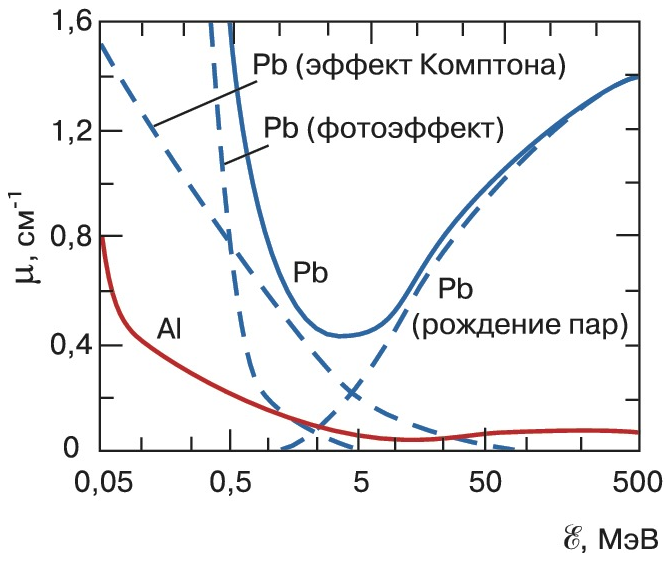
\includegraphics[scale=0.35]{img/mu}}
	\caption{Линейные коэффициенты ослабления для фотоэффекта, эффекта Комптона и образования электрон-позитронных пар от энергии \(\gamma\)-квантов}
	\label{img:mu}
\end{figure}

\subsubsection{Фотоэффект} 

Данный эффект заключается в поглощении атомом падающего на него фотона с энергией \(\varepsilon =\hbar\omega\) с последующим испусканием одного из связанных на \(i\)-й оболочке электронов. Из законов сохранения энергии и импульса следует, что фотоэффект не может происходить на свободном электроне. Фотоэффект возможен на любой электронной оболочке, однако электроны \(K\)-оболочки испускаются с большей вероятностью, по сравнению с более отдаленными от ядра оболочками.

Энергия вылетевшего электрона определяется как разность энергии налетающего фотона и энергии связи электрона \(i\)-ой оболочки с ядром:
\begin{equation}\label{eq:photo_eff}
E_e=\varepsilon-A
\end{equation}

\subsubsection{Эффект Комптона} 

Суть данного процесса заключается в изменении энергии фотона при его упругом столкновении с электроном. В результате соударения фотон теряет часть своей энергии и, как следствие, длина его волны увеличивается. Процесс происходит на свободных или слабосвязанных электронах в присутствии третьего тела для удовлетворения законов сохранения энергии и импульса. Изменение энергии фотона при эффекте Комптона описывается следующей формулой:

\begin{equation}\label{eq2}
E_{\gamma '}= \frac{E_{\gamma}}{1+(E_{\gamma}/m_ec^{2})(1-\cos\theta)},
\end{equation}

где \(E_{\gamma}\) "--- энергия падающего кванта, \(E_{\gamma '}\) -- энергия рассеянного кванта, \(\theta\) "--- угол рассеяния.

\subsubsection{Образование электрон-позитронной пары} 

Образование электрон-позитронной пары является результатом взаимодействия фотона с электромагнитным полем атома вблизи ядра. Данный процесс возможен только для тех фотонов, чья энергия превышает порог образования электрона и позитрона:

\begin{equation}\label{eq3}
	h\nu_\text{порог}=2m_0c^2=1.022 \ \text{МэВ}\ ,
\end{equation}
где \(\nu_\text{порог}\) "--- частота падающего фотона, \(m_0\) "--- масса покоя электрона.
